\newpage
\section{Part F}
\label{sec:sec_f}

In this experiment we sweep two different optimizers (\textbf{Adam} and \textbf{SGD}) across different number of training epochs. Figure~\ref{fig:f} compares the final training loss after $X$ epochs and the training time. For this experiment training was ran entirely on the CPU.

\LST{part\_f}

It can be seen that with a large number of Epochs the \textit{Adam} optimizer does eventually converge towards the same values as the \textit{SGD} optimizer. And the ADAM runtime is slightly slower.

\begin{figure}[htpb]
	\centering
	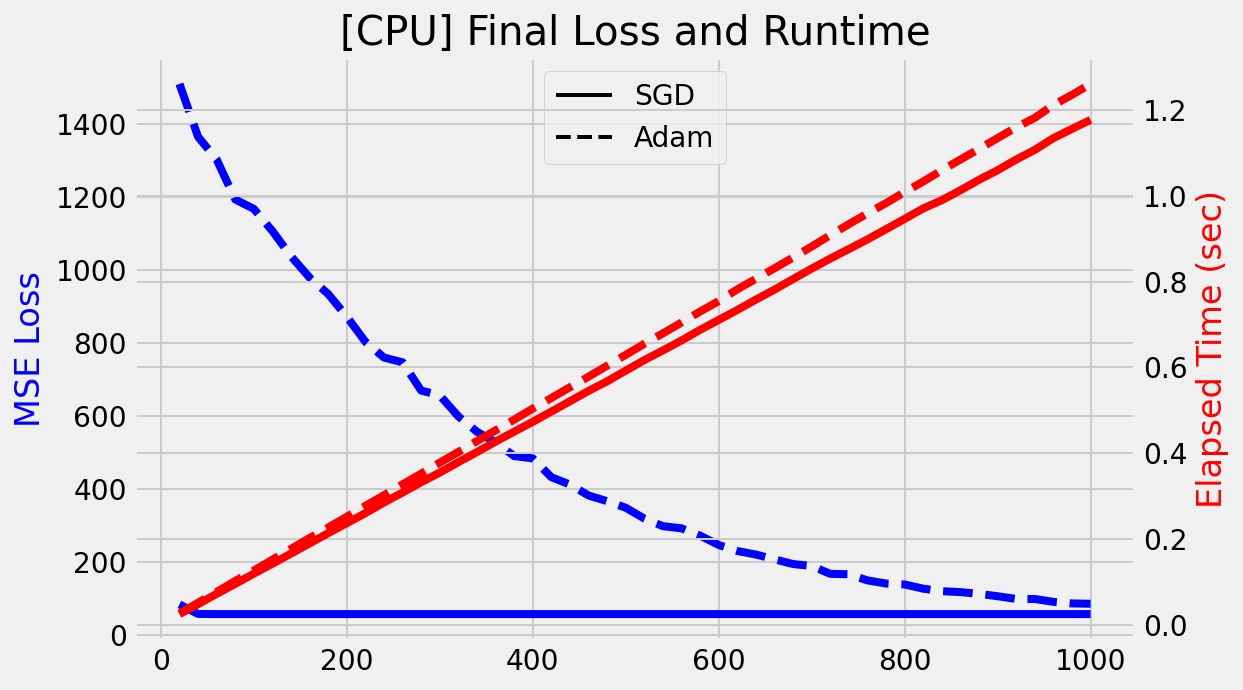
\includegraphics[width=\columnwidth]{figures/cpu_timing.png}
	\caption{CPU Final Training loss and Runtime vs Epochs}
	\label{fig:f}
\end{figure}


